% SVN info for this file
\svnidlong
{$HeadURL$}
{$LastChangedDate$}
{$LastChangedRevision$}
{$LastChangedBy$}

\chapter{Analisi e probabilità}
\labelChapter{analisiprobabilità}

\begin{introduction}
	‘‘Se il tuo esperimento richiede di usare la statistica, dovevi fare un esperimento migliore.''
	\begin{flushright}
		\textsc{Ernest Rutherford,} stanco di studiare Calcolo delle Probabilità e Statistica.
	\end{flushright}
\end{introduction}
\lettrine[findent=1pt, nindent=0pt]{C}{ome} abbiamo potuto notare nel corso di \textsc{Calcolo di Probabilità}, la teoria della \textbf{probabilità} si è notevolmente espansa dal mero studio di eventi discreti con metodi combinatoriali. Infatti, Andrey Nikolaevich \textbf{Kolmogorov} (1903 – 1987) nel 1933 combinò la nozione di spazio campione, già introdotta da Richard \textbf{von Mises} (1883 – 1953), e la teoria della misura di Lebesgue per definire un sistema assiomatico compatibile sia con la teoria \textit{classica} della probabilità, sia con l'\textit{Analisi moderna}: in questo modo, gli eventi potevano essere anche un qualcosa di \textit{continuo}, con tutto ciò che ne consegue.\\
In questo ultimo capitolo di teoria approfondiremo alcuni concetti visti a \textsc{Calcolo di Probabilità} con il formalismo e il rigore dato dalla teoria della Misura e dell'integrazione. Partiremo con l'enunciare gli \textit{assiomi di probabilità} di Kolmogorov per poi dedicarci a come studiare le \textit{variabili aleatorie} tramite la sola \textit{probabilità immagine}, e in base ad essa dare una classificazione \textit{esaustiva} delle variabili aleatorie. Concludiamo la trattazione rivedendo i \textit{modi di convergenza} delle funzioni misurabili in ambito probabilistico.
\section{Spazio di probabilità e variabili aleatorie}
\begin{define}[Spazio di probabilità]
	Uno \textbf{spazio di probabilità}\index{spazio!di probabilità} $\left(\Omega,\mathcal{F},\mathbb{P}\right)$ è una struttura matematica che fornisce un modello formale per un esperimento non deterministico. Essa costituita dai seguenti elementi:
	\begin{enumerate}
		\item Uno \textbf{spazio campionario}\index{spazio!campionario} $\Omega$, l'insieme di tutti i possibili \textbf{risultati} $\omega$ dell'esperimento.
		\item Uno \textbf{spazio degli eventi}\index{spazio!degli eventi} $\mathcal{F}$, la famiglia di tutti gli eventi dell'esperimento, dove un \textbf{evento}\index{evento} $E$ è un insieme di risultati dello spazio campionario - ossia un sottoinsieme di $\Omega$.
		\item Una \textbf{funzione di probabilità} $\mathbb{P}$, che assegna ad ogni evento una probabilità, la quale è un numero tra 0 e 1.
		\begin{equation}
			\funz{\mathbb{P}}{\mathcal{F}}{\left[0,1\right]}
		\end{equation}
	\end{enumerate}
\end{define}
Questo spazio di probabilità deve soddisfare gli assiomi di probabilità introdotti da Andrey Kolmogorov nel 1933.
\begin{axiom}[Primo assioma di probabilità]
	La probabilità di un evento è un numero reale non negativo.
	\begin{equation}
		\mathbb{P}\left(E\right)\in\realset,\ \mathbb{P}\left(E\right)\geq 0\quad \forall E\in\mathcal{F} 
	\end{equation}
\end{axiom}
\begin{axiom}[Secondo assioma di probabilità]
	La probabilità dello spazio campionario è $1$.
	\begin{equation}
		\mathbb{P}\left(\Omega\right)=1
	\end{equation}
\end{axiom}
\begin{axiom}[Terzo assioma della probabilità]
	La probabilità è $\sigma$-additiva:	$\forall A_n\in\mathcal{F}$ tali che $A_i\cap A_j=\emptyset\ \forall i\neq j$, allora
	\begin{equation}
		\mathbb{P}\left(\coprod_{n\geq 1}A_n\right)=\sum_{n\geq 1}\mathbb{P}\left(A_n\right)
	\end{equation}
\end{axiom}
\begin{proposition}[L'insieme vuoto ha probabilità nulla]
	Sia $\left(\Omega,\mathcal{F},\mathbb{P}\right)$ uno spazio di probabilità. Allora l'insieme vuoto ha probabilità nulla.
\end{proposition}
\begin{demonstration}
	Consideriamo la successione di eventi seguente:
	\begin{equation*}
		A_n=\begin{cases}
			\begin{array}{ll}
				\Omega&n=1\\
				\emptyset&n\geq2
			\end{array}
		\end{cases}
	\end{equation*}
	Osserviamo che $\Omega\cap \emptyset=\emptyset$ e $\emptyset\cap\emptyset=0$; poiché
	\begin{equation*}
		\Omega=\bigcup_{n\geq 1}A_n,
	\end{equation*}
	applichiamo l'assioma 3, la $\sigma$-additività all'unione degli $A_n$:
	\begin{align*}
		1&=\mathcal{P}\left(\Omega\right)=\mathcal{P}\left(\bigcup_{n\geq 0}A_n\right)=\sum_{n\geq 1}\mathbb{P}\left(A_n\right)=\mathbb{P}\left(A_1\right)+\sum_{n\geq2}\mathbb{P}\left(A_n\right)&\\
		&=\mathbb{P}\left(\Omega\right)+\sum_{n\geq 2}\mathbb{P}\left(\emptyset\right)&\text{(Assioma 1)}\\
		&=1-\sum_{n\geq 2}\mathbb{P}\left(\emptyset\right)&
	\end{align*}
	da cui
	\begin{equation*}
		\sum_{n\geq 2}\mathbb{P}\left(\emptyset\right)=0
	\end{equation*}
	Poiché per il primo assioma la probabilità di un evento è sempre non-negativa, ne consegue che ogni elemento di questa sommatoria debba essere uguale a zero, ossia $\mathcal{P}\left(\emptyset\right)=0$.
\end{demonstration}
Si può subito osservare che lo spazio di probabilità $\left(\Omega,\mathcal{F},\mathbb{P}\right)$ altro non è che uno \textbf{spazio di misura} $\left(X,\mathcal{M},\mu\right)$, con l'ipotesi aggiunta che la misura $\mu$ sia di \textbf{probabilità}, cioè $\mu(X)=1$.
\begin{define}[Funzione misurabile]
	Sia $\left(\Omega,\mathcal{F},\mathbb{P}\right)$ uno spazio di probabilità. Una funzione $\funz{X}{\Omega}{\complexset}$ si dice \textbf{variabile aleatoria}\index{variabile aleatoria} se \begin{equation}
		X^{-1}\left(A\right)\in\mathcal{F},\ \forall A\subseteq \complexset\text{ aperto.}
	\end{equation}
\end{define}
In altre parole, una variabile aleatoria è una funzione misurabile da uno spazio di probabilità a $\complexset$.
\section{Probabilità immagine}\label{probimm}
Nel corso di \textsc{Calcolo di Probabilità} abbiamo incontrato la variabile aleatoria \textbf{normale standard} $Z$, definita come tale se la probabilità che $Z$ stia nell'evento $B$ è
\begin{equation}
	\mathbb{P}\left(Z\in B\right)=\int_{B}\frac{1}{\sqrt{2\pi}}e^{-x^2/2}dm_1,\ \forall B\in\mathcal{B}\left(\realset\right)
\end{equation}
Le variabili aleatorie, per definizione, sono funzioni da uno spazio di probabilità $\Omega$ a valori - in questo caso - reali. La definizione della normale standard, tuttavia, non fa alcun riferimento allo spazio di probabilità. Cos'è dunque  $\left(\Omega,\mathcal{F},\mathbb{P}\right)$?\\
In realtà \textit{non si sa}, ma non ci interessa individuarlo. Motiviamo questa affermazione audace introducendo il concetto di \textit{misura immagine}, visto nell'ambito di Teoria della probabilità come \textit{probabilità immagine}.
\begin{define}[Misura immagine]
	Siano $\left(X,\mathcal{F}\right)$ e $\left(Y,\mathcal{M}\right)$ due spazi misurabili e una funzione $\funz{f}{X}{Y}$ misurabile. Se su $\left(X,\mathcal{F}\right)$ consideriamo una misura $\funz{\mu}{\mathcal{F}}{\left[0,+\infty\right]}$, la \textbf{misura immagine}\index{misura!immagine} o \textbf{pushforward}\index{misura!pushforward} è la misura $\funz{f_{\ast}\left(\mu\right)}{\mathcal{M}}{\left[0,+\infty\right]}$ definita da
	\begin{equation}
		\left[f_{\ast}\left(\mu\right)\right]\left(B\right)=\mu\left(f^{-1}\left(B\right)\right),\ \forall B\in \mathcal{M}
	\end{equation}
\end{define}
\begin{theoremaqed}[Integrazione con cambio di variabili tramite pushforward]
	Data una funzione $g$ su $Y$ misurabile, allora
	\begin{equation}
		g\in L^{1}\left(f_{\ast}\left(\mu\right)\right)\iff g\circ f\in L^{1}\left(\mu\right),
	\end{equation}
	ossia
	\begin{equation}
		\int_{X}g\circ fd\mu=\int_{Y}gd\left(f_{\ast}\left(\mu\right)\right)\qedhere
	\end{equation}
\end{theoremaqed}
Interpretiamo questo nuovo concetto nell'ambito degli spazi di probabilità.
\begin{define}[Probabilità immagine]
	Sia $\left(X,\mathcal{M},\mathbb{P}\right)$ e spazio di probabilità e $\funz{X}{\Omega}{\realset}$ variabile aleatoria.
	La \textbf{probabilità immagine}\index{probabilità!immagine} è la misura di probabilità $\funz{\mathbb{P}_X}{\mathcal{B}\left(\realset\right)}{\left[0,1\right]}$ definita da
	\begin{equation}
		\mathbb{P}_X\left(B\right)=\mathbb{P}\left(X^{-1}\left(B\right)\right),\ \forall B\in \mathcal{B\left(\realset\right)}
	\end{equation}
	e definisce un nuovo spazio di probabilità $\left(\realset,\mathcal{B}\left(\realset\right),\mathbb{P}_X\right)$.
\end{define}
\begin{theoremaqed}[Integrazione con cambio di variabili tramite probabilità immagine]
	Data una funzione $g$ su $\realset$ misurabile, allora
	\begin{equation}
		\circled[blue]{\spadesuit}\quad g\in L^{1}\left(\mathbb{P}_X\right)\iff g\circ X\in L^{1}\left(\mathbb{P}\right),
	\end{equation}
	ossia
	\begin{equation}
		\int_{\Omega}g(x)d\mathbb{P}=\int_{\realset}gd\mathbb{P}_X\qedhere
	\end{equation}
\end{theoremaqed}
\begin{center}
	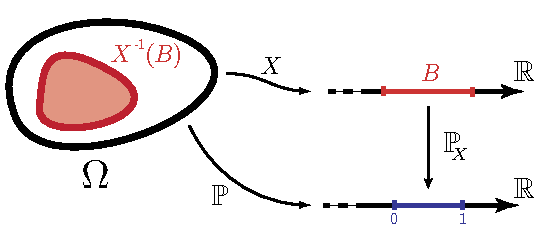
\includegraphics[width=0.4\paperwidth]{images/probimmagine}
\end{center}
Pertanto, non mi interessa nello specifico sapere cos'è $\Omega$ o com'è definita $\mathbb{P}$: se definisco la variabile aleatoria direttamente con la probabilità immagine ‘‘dimentico'' quale fosse lo spazio originale e lavoro direttamente su $\realset$.
\begin{define}[Momento di ordine {$k$-esimo}]
	Se consideriamo la funzione $g(x)=x^k,\ \forall x\in\realset$ e $\forall k\in\naturalset$, si definisce il \textbf{momento}\index{momento di ordine {$k$}-esimo} il valore
	\begin{equation*}
		\mathbb{E}\left(X^k\right)=\int_{\Omega}X^kd\mathbb{P}=\int_{\realset}x^kd\mathbb{P}_X
	\end{equation*}
\end{define}
\section{Funzione di ripartizione e classificazione delle variabili aleatorie}
\begin{define}[Funzione di ripartizione]
	Siano $\left(\Omega,\mathcal{M},\mathbb{P}\right)$ uno spazio di probabilità, $\funz{X}{\Omega}{\realset}$ una variabile aleatoria e $\mathbb{P}_X$ la corrispondente probabilità immagine. Si chiama \textbf{funzione di ripartizione}\index{funzione!di ripartizione} (abbreviata in \textbf{cdf}, dall'inglese \textit{cumulative distributive function}) la funzione $\funz{F_X}{\realset}{\left[0,1\right]}$ definita da
	\begin{equation}
		F_X(x)=\mathbb{P}_X\left(\left(-\infty,x\right]\right)=\mathbb{P}\left(X\leq x\right),\ \forall x\in\realset
	\end{equation}
\end{define}
Una funzione di ripartizione $F_X$ soddisfa le seguenti proprietà:
\begin{enumerate}
	\item È monotona non decrescente.
	\item È continua a destra.
	\item È tale per cui
	\begin{equation}
		\lim_{x\to+\infty}F_X(x)=0\quad\lim_{x\to+\infty}F_X(x)=1
	\end{equation}
	ossia ha immagine $\left[0,1\right]$.
\end{enumerate}
Vale anche il viceversa: una funzione che soddisfa queste caratteristiche è una funzione di ripartizione per qualche variabile aleatoria.\\
La variabili aleatorie si classificano in base alla probabilità immagine $\mathbb{P}_X$ e, di conseguenza, alla funzione di ripartizione $F_X$, in una delle quattro classi seguenti:
\begin{itemize}
	\item V.a. \textit{assolutamente continue}.
	\item V.a. \textit{singolari discrete}.
	\item V.a. \textit{singolari continue}.
	\item V.a. \textit{miste}.
\end{itemize}
\subsection{Variabili aleatorie assolutamente continue}
\begin{define}[V.a. assolutamente continua e densità]
	$X$ si dice variabile aleatoria \textbf{assolutamente continua}\index{variabile aleatoria!assolutamente continua} se $\mathbb{P}_X$ è assolutamente continua rispetto alla misura di Lebesgue $m_1$:
	\begin{equation}
		\forall E\in\mathcal{B}\left(\realset\right),\ m_1\left(E\right)=0\implies \mathbb{P}_X\left(E\right)=0
	\end{equation}
	Per il \textit{teorema di Radon-Nikodym} esiste quindi una funzione detta \textbf{densità} $f\in\mathcal{L}^1\left(\realset\right)$, $f\geq 0$ tale che
	\begin{equation}
		\mathbb{P}_X\left(B\right)=\int_B fdm_1,\ \forall B\in\mathcal{B}\left(\realset\right)
	\end{equation}
\end{define}
Abbiamo già visto\footnote{Si veda \refChapterOnly{integraledilebesgue}, pag. \pageref{misuraindotta}.} come integrare delle funzioni rispetto ad una misura indotta da un'altra misura, come qui è il caso.
\begin{theoremaqed}[Integrazione di funzioni rispetto a v.a. assolutamente continue]
	Data una funzione $g$ su $\realset$, allora
	\begin{equation}
		g\in L^{1}\left(\mathbb{P}_X\right)\iff fg\in L^{1}\left(m_1\right),
	\end{equation}
	ossia
	\begin{equation}
		\int_{\realset}gd\mathbb{P}_X=\int_{\realset}fgdm_1\qedhere
	\end{equation}
\end{theoremaqed}
\begin{define}[Momento di una ordine {$k$-esimo} di v.a. assolutamente continue]
	Sia $X$ una v.a. assolutamente continua di densità $f$. Se consideriamo la funzione $g(x)=x^k,\ \forall x\in\realset$ e $\forall k\in\naturalset$, si definisce il \textbf{momento}\index{momento di ordine {$k$}-esimo} il valore
	\begin{equation*}
		\mathbb{E}\left(X^k\right)=\int_{\Omega}X^kd\mathbb{P}=\int_{\realset}x^kd\mathbb{P}_X=\int_{\realset}x^kd\mathbb{P}_X=\int_{\realset}x^kfdm_1
	\end{equation*}
\end{define}
\begin{examplewt}[Variabile aleatoria normale]
	Approfondendo ciò ad inizio della sezione \ref{probimm}. La variabile aleatoria \textbf{normale standard}\index{variabile aleatoria!normale standard} è una variabile aleatoria $\funz{Z}{\Omega}{\realset}$ di cui è ignoto lo spazio di probabilità $\left(\Omega,\mathcal{M},\mathbb{P}\right)$; tuttavia, essa è definita attraverso la probabilità immagine $\mathbb{P}_X$ assolutamente continua rispetto alla misura $m_1$ associata alla densità Gaussiana:
	\begin{equation}
		\mathbb{P}\left(X\in\mathbb{B}\right)=\mathbb{P}_X\left(B\right)=\int_B\frac{1}{\sqrt{2\pi}}e^{-x^2/2}dm_1,\ \forall B\in\mathcal{B}\left(\realset\right)
	\end{equation}
	I momenti della v.a. normale standard sono
	\begin{equation*}
		\mathbb{E}X^k=\int_{\Omega}X^kd\mathbb{P}=\int_{\realset}x^kd\mathbb{P}_X=\int_{\realset}x^k\frac{1}{\sqrt{2\pi}}e^{-x^2/2}dm_1
	\end{equation*}
\end{examplewt}
\paragraph{Cdf di v.a. assolutamente continue}
La funzione di ripartizione $\funz{F_X}{\realset}{\left[0,1\right]}$ di una variabile aleatoria assolutamente continua è una funzione \textbf{assolutamente continua}.
\begin{center}
	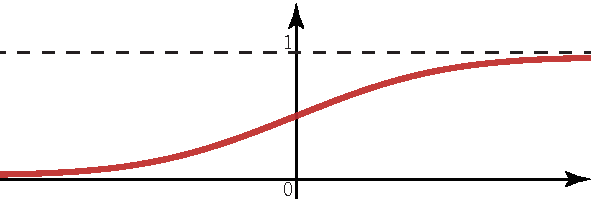
\includegraphics[width=0.4\paperwidth]{images/vacontinua}
\end{center}
\begin{define}[Assoluta continuità.]
	Una funzione $\funz{f}{\realset}{\realset}$ è assolutamente continua se
	\begin{gather*}
		\forall \epsilon>0,\ \exists \delta >0\colon \forall \left(a_1,b_1\right),\ \dots,\ \left(a_n,b_n\right),\ \left(a_i,b_i\right)\cap\left(a_j,b_j\right)=\emptyset,\ \forall i\neq j,\\
		\sum_{i=1}^{n}\abs{b_i-a_i}<\delta\implies\sum_{i=1}^{n}\abs{f\left(b_i\right)-f\left(a_i\right)}<\epsilon
	\end{gather*}
\end{define}
\begin{observe}
	Scegliendo un unico intervallo $\left(a_1,b_1\right)$ si ritrova la definizione di \textit{uniforme continuità}. Pertanto, l'assoluta continuità è una condizione più forte dell'uniforme continuità e in quanto tale implica anche la continuità della funzione originale.
\end{observe}
Ricordiamo che
\begin{equation*}
	F_X(x)=\mathbb{P}_X\left(\left(-\infty,x\right]\right)=\int_{\left(-\infty,x\right]}fdm_1
\end{equation*}
Si dimostra che $F_X$ è derivabile \textbf{q.o.} e che vale
\begin{equation}
	F'_X(x)=f(x),\ \textrm{per quasi ogni }x\in\realset
\end{equation}
Questa relazione non è altro che l'\textbf{estensione del teorema fondamentale del calcolo integrale alla teoria di Lebesgue}\index{teorema!fondamentale del calcolo integrale nella teoria di Lebesgue}.
\subsection{Misure singolari}
Consideriamo una misura $\funz{\lambda}{\mathcal{B}\left(\realset\right)}{\left[0,+\infty\right]}$ non assolutamente continua rispetto alla misura di Lebesgue $m_1$.
Negare
\begin{equation*}
	\forall E\in\mathcal{B}\left(\realset\right)\colon m_1\left(E\right)=0\implies \lambda\left(E\right)=0
\end{equation*}
significa che esiste un insieme $S\in\mathcal{B}\left(\realset\right)$ tale che
\begin{equation*}
	m_1\left(S\right)=0\text{ ma }\lambda\left(S\right)\neq 0
\end{equation*}
In particolare, se vale
\begin{equation*}
	\lambda\left(S\right)=\lambda\left(\realset\right)
\end{equation*}
la misura viene chiamata \textit{singolare} e si definisce \textit{concentrata} in $S$
\begin{define}[Misura singolare]
	Dato un spazio di misura $\left(X,\mathcal{M},\mu\right)$, una misura $\funz{\lambda}{\mathcal{M}}{\left[0,+\infty\right]}$ non assolutamente continua rispetto a $\mu$ si dice \textbf{singolare}\index{misura!singolare} rispetto a $\mu$ se
	\begin{equation}
		\exists S\in\mathcal{M}\colon \mu\left(S\right)=0, \lambda\left(S\right)\neq0 \text{ ma }\lambda(X)=\lambda\left(S\right)
	\end{equation}
	La misura $\lambda$ è detta \textbf{concentrata} in $S$ e si indica con $\mu\perp\lambda$.
	\begin{itemize}
		\item Se $\lambda$ è concentrata in $S$ insieme numerabile, allora $\lambda$ è detta \textbf{singolare discreta}\index{misura!singolare!discreta} o \textbf{atomica}\seeonlyindex{misura!singolare!atomica}{misura!singolare!discreta}.
		\item Se $\lambda$ è concentrata in $S$ insieme \textit{non} numerabile, $\lambda$ è detta \textbf{singolare continua}\index{misura!singolare!continua}.
	\end{itemize}
\end{define}
\begin{observe}
	Si può vedere che se prendo $A\subseteq S^{C}=X\setminus S$, allora $\lambda\left(A\right)=0$, in quanto se così non fosse si avrebbe $\lambda\left(S\right)\neq\lambda(X)$. Si osserva chiaramente che vale anche il viceversa per $\mu$: se prendo $B\subseteq S$, allora $\mu\left(B\right)=0$.\\
	Da ciò, si vede una definizione alternativa per le misura singolari: una misura $\lambda$ singolare rispetto a $\mu$ se esiste un insieme $S\in\mathcal{M}$ tale che $\mu\left(A\right)=0,\ \forall A\subseteq S$ misurabili e $\lambda\left(B\right)=0,\ \forall A\subseteq S^{C}$ misurabili.
\end{observe}
\subsection{Variabili aleatorie singolari discrete}
\begin{define}[Variabili aleatorie singolari discrete]
	$X$ si dice variabile aleatoria \textbf{singolare discreta}\index{variabile aleatoria!singolare!discreta} o \textbf{atomica}\seeonlyindex{variabile aleatoria!singolare!atomica}{variabile aleatoria!singolare!discreta} se $\mathbb{P}_X$ è \textbf{singolare discreta} rispetto alla misura di Lebesgue $m_1$.\\
	Per definizione di misura singolare discreta, esiste $S=\left\{\omega_n\right\}_{n\geq 1}$ tale che, posto
	\begin{equation}
		p_n=\mathbb{P}_X\left(\left\{\omega_n\right\}\right),\ \forall n\geq 1,
	\end{equation}
	si ha
	\begin{equation}
		\mathbb{P}\left(B\right)=\sum_{n\colon\omega_n\in B}p_n,\ \forall B\in\mathcal{B}\left(\realset\right)
	\end{equation}
\end{define}

\begin{theoremaqed}[Integrazione di funzioni rispetto a v.a. singolari discrete]
	Data una funzione $g$ su $\realset$, allora
	\begin{equation}
		g\in L^{1}\left(\mathbb{P}_X\right)\iff \sum_{n=1}^{+\infty}\abs{g\left(\omega_n\right)}p_n<+\infty
	\end{equation}
	e
	\begin{equation}
		\int_{\realset}gd\mathbb{P}_X=\sum_{n=1}^{+\infty}g\left(\omega_n\right)p_n\qedhere
	\end{equation}
\end{theoremaqed}
Abbiamo già dimostrato questo teorema parlando dell'integrazione rispetto ad una misura conteggio pesata\footnote{Si veda \refChapterOnly{integraledilebesgue}, teorema \ref{integrazionemisuraconteggiopesata}, pag. \pageref{integrazionemisuraconteggiopesata}.}.
\paragraph{Cdf di v.a. singolari discrete}
La funzione di ripartizione $\funz{F_X}{\realset}{\left[0,1\right]}$ di una variabile aleatoria singolare discreta è una funzione \textbf{costante a tratti}.
\begin{center}
	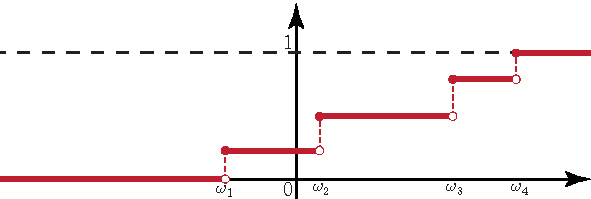
\includegraphics[width=0.4\paperwidth]{images/vadiscreta}
\end{center}
In particolare, $S$ è l'insieme delle discontinuità di $F_X$ e vale
\begin{equation}
	p_n=\lim_{x\to\omega_n^{+}}F_X(x)-\lim_{n\to\omega_n^{-}}F_X(x),\ \forall n\geq 1
\end{equation}
\subsection{Variabili aleatorie singolari continue}
\begin{define}[Variabili aleatorie singolari continue]
	$X$ si dice variabile aleatoria \textbf{singolare continua}\index{variabile aleatoria!singolare!continua} se $\mathbb{P}_X$ è \textbf{singolare continua} rispetto alla misura di Lebesgue $m_1$.\\
	Per definizione di misura singolare continua, esiste $S$ non numerabile con misura di Lebesgue nulla tale che,
	\begin{equation}
		\mathbb{P}_X\left(S\right)=1
	\end{equation}
\end{define}
\paragraph{Cdf di v.a. singolari continua}
La funzione di ripartizione $\funz{F_X}{\realset}{\left[0,1\right]}$ di una variabile aleatoria singolare continua è una funzione \textbf{continua} ma non \textit{assolutamente continua}.\\
In particolare, si dimostra che $F_X$ è derivabile su $\realset\setminus S$ (ossia \textbf{q.o.}) e
\begin{equation}
	F'_X(x)=0,\ \forall x\in\realset\setminus S
\end{equation}
\begin{observe}
	Questa condizione è compatibile con il fatto che $F_X$ sia crescente ed abbia come immagine $\left[0,1\right]$.
\end{observe}
\begin{examplewt}[Distribuzione di Cantor]
Una funzione ha la \textbf{distribuzione di Cantor}\index{distribuzione!di Cantor} se la sua funzione di ripartizione è la \textit{funzione di Cantor}\footnote{Si veda \refChapterOnly{teoriamisura}, teorema \ref{funzionecantor}, pag. \pageref{funzionecantor}.}.
\begin{center}
	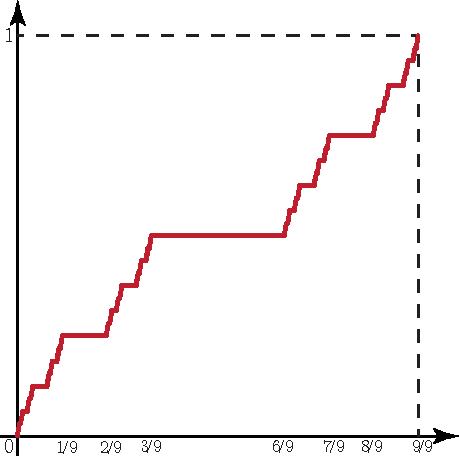
\includegraphics[width=0.4\paperwidth]{images/vasingolarecontinua}
\end{center}
Per quanto detto su tale funzione, essa soddisfa tutte le condizioni di essere la cdf di una variabile aleatoria singolarmente continua. In quanto tale, questa variabile aleatoria non ammette una funzione di densità, ma si può vedere, per simmetria.
\end{examplewt}
\subsection{Variabili aleatorie qualsiasi}
Abbiamo elencato tre diverse classi di misure di probabilità e variabili aleatorie ad esse associate. Il seguente teorema ci permette di affermare che esiste solo un'ulteriore classe di misure e variabili, le quali tuttavia non sono altro che combinazioni dei tre tipi precedentemente enunciati.
\begin{theoremaqed}[Teorema di Radon-Nikodym-Lebesgue]\index{teorema!di Radon-Nikodym-Lebesgue}
	Sia $\funz{\mathbb{P}}{\mathcal{B}\left(\realset\right)}{\left[0,1\right]}$ una misura di probabilità. Allora esistono $\alpha_1,\ \alpha_2,\ \alpha_3\geq 0$ e tre misure di probabilità $\mathbb{P}^{ac},\ \mathbb{P}^{sd},\ \mathbb{P}^{sc}$ assolutamente continua, singolare discreta e singolare continua, rispettivamente, tali che
	\begin{equation}
		\mathcal{P}=\alpha_1\mathbb{P}^{ac}+\alpha_2\mathbb{P}^{sd}+\alpha_3\mathbb{P}^{sc}\qedhere
	\end{equation}
\end{theoremaqed}
Come conseguenza, ogni variabile aleatoria si decompone nella somma di tre variabili aleatorie, una assolutamente continua, una discreta e una singolare continua.
\section{Modi di convergenza nella teoria della probabilità}
Come abbiamo potuto notare, la teoria assiomatica della probabilità è profondamente legata alla teoria della misura. Nella sezione \ref{modiconvergenza} abbiamo visto diversi modi in cui una successione di funzioni misurabili $\funz{f_n}{X}{\complexset}$ poteva convergere ad una funzione limite misurabile $\funz{f}{X}{\complexset}$. Studiamo ora i modi di convergenza di una successione di variabili aleatorie $\funz{X_n}{\Omega}{\complexset}$ ad una variabile aleatoria limite $\funz{X}{\Omega}{\complexset}$.
\paragraph{Convergenza puntuale o convergenza certa}
\begin{define}[Convergenza puntuale o convergenza certa]
	Consideriamo lo spazio di probabilità $\left(\Omega,\mathcal{F},\mathbb{P}\right)$ e le variabili aleatorie $\funz{X_n,X}{\Omega}{\complexset}$
	Si dice che $X_n$ \textbf{converge certamente}\index{convergenza!certa} a $X$\textbf{su} $\Omega$ ($X_n\overset{\text{c.}}{\to} X$) se
	\begin{equation}
		\lim_{n\to+\infty}X_n\left(\omega\right)=X\left(\omega\right),\ \forall \omega\in\Omega
	\end{equation}
\end{define}
La convergenza certa implica tutti i modi di convergenza successivi, ma \textit{non c'è alcun vantaggio} ad usare questa convergenza rispetto alla convergenza quasi certa.
\paragraph{Convergenza quasi certa}
\begin{define}[Convergenza quasi certa]
	Consideriamo lo spazio di probabilità $\left(\Omega,\mathcal{F},\mathbb{P}\right)$ e le variabili aleatorie $\funz{X_n,X}{\Omega}{\complexset}$
	Si dice che $X_n$ \textbf{converge quasi certamente}\index{convergenza!quasi certa} a $X$\textbf{su} $\Omega$ ($X_n\overset{\text{q.c.}}{\to} X$) se
	\begin{equation}
		\mathbb{P}\left(\left\{\omega\in\Omega \ \middle| \ \lim_{n\to+\infty}X_n\left(\omega\right)=X\left(\omega\right)\right\}\right)=1
	\end{equation}
\end{define}
Osserviamo che in uno spazio di probabilità $\left(\Omega,\mathcal{F},\mathbb{P}\right)$ questa convergenza è equivalente alla convergenza \textit{quasi ovunque}. Infatti:
\begin{align*}
	\left\{\omega\in \Omega\middle|\lim_{n\to+\infty}X_n\left(\omega\right)\neq X\left(\omega\right)\right\}&=\Omega\setminus\left\{\omega\in \Omega\middle|\lim_{n\to+\infty}X_n\left(\omega\right)= X\left(\omega\right)\right\}\\
	\mathbb{P}\left(\left\{\omega\in \Omega\middle|\lim_{n\to+\infty}X_n\left(\omega\right)\neq X\left(\omega\right)\right\}\right)&\underset{\mathbb{P}(x)<+\infty}{=}\mathbb{P}\left(\Omega\right)-\mathbb{P}\left(\left\{\omega\in \Omega\middle|\lim_{n\to+\infty}X_n\left(\omega\right)= X\left(\omega\right)\right\}\right)\\
	\mathbb{P}\left(\left\{\omega\in \Omega\middle|\lim_{n\to+\infty}X_n\left(\omega\right)\neq X\left(\omega\right)\right\}\right)&=1-\mathbb{P}\left(\left\{\omega\in \Omega\middle|\lim_{n\to+\infty}X_n\left(\omega\right)= X\left(\omega\right)\right\}\right)
\end{align*}
Allora affermare che
\begin{equation*}
	\mathbb{P}\left(\left\{\omega\in \Omega \ \middle| \ \lim_{n\to+\infty}X_n\left(\omega\right)= X\left(\omega\right)\right\}\right)=1
\end{equation*}
significa affermare che
\begin{equation*}
	\mathbb{P}\left(\left\{\omega\in \Omega \ \middle| \ \lim_{n\to+\infty}X_n\left(\omega\right)\neq X\left(\omega\right)\right\}\right)=0
\end{equation*}
\begin{attention}
	In uno spazio di misura che \textit{non} sia di probabilità questa corrispondenza non si può fare, dato che $\mu(X)$ può non essere pari ad $1$, tanto meno finito. Vale sempre la convergenza \textbf{q.o.}, ma mai quella \textbf{q.c.}.
\end{attention}
\newpage
\paragraph{Convergenza in probabilità}
\begin{define}[Convergenza in probabilità]
	Consideriamo lo spazio di probabilità $\left(\Omega,\mathcal{F},\mathbb{P}\right)$ e le variabili aleatorie $\funz{X_n,X}{\Omega}{\complexset}$. Si dice che	$X_n$ \textbf{converge in probabilità}\index{convergenza!in probabilità} a $X$ ($X_n\overset{\mathbb{P}}{\to} X$) se
	\begin{equation}
		\lim_{n\to+\infty}\mu\left(\left\{\omega\in \Omega\mid \abs{X_n\left(\omega\right)-X\left(\omega\right)}<\epsilon\right\}\right)=1,\ \forall \epsilon >0
	\end{equation}
\end{define}
In modo analogo alla convergenza quasi certa, in uno spazio di probabilità $\left(\Omega,\mathcal{F},\mathbb{P}\right)$ questa convergenza è equivalente alla \textit{convergenza in misura}.
\begin{attention}
	In uno spazio di misura che \textit{non} sia di probabilità questa corrispondenza non si può fare, dato che $\mu(X)$ può non essere pari ad $1$, tanto meno finito. Vale sempre la convergenza in misura, ma mai quella in probabilità.
\end{attention}
\paragraph{Convergenza in media}
\begin{define}[Convergenza in media]
	Consideriamo lo spazio di probabilità $\left(\Omega,\mathcal{F},\mathbb{P}\right)$ e le variabili aleatorie $\funz{X_n,X}{\Omega}{\complexset}$. Si dice che
	$X_n$ \textbf{converge in media}\index{convergenza!in media} a $f$ ($X_n\overset{L^1}{\to} X$) se
	\begin{equation}
		\lim_{n\to+\infty}\mathbb{E}X_n=\mathbb{E}X
	\end{equation}
	o, equivalentemente, se passiamo alla probabilità immagine,
	\begin{equation}
		\lim_{n\to+\infty}\int_\realset X_nd\mathbb{P}_Y=\int_{\realset}Xd\mathbb{P}_Y
	\end{equation}
\end{define}
\paragraph{Convergenza in legge}
\begin{define}[Convergenza in legge]
	Dato $\left(\Omega,\ \mathcal{M},\ \mathbb{P}\right)$ spazio di probabilità e le variabili aleatorie $\funz{X_n,\ X}{\Omega}{\realset}$ con le corrispettive \textit{funzioni di distribuzione}
	\begin{gather*}
		\funztot{F_n}{\realset}{\realset}{x}{F_n(x)=\mathbb{P}\left(X_n\leq x\right),\ \forall x\in \realset}\\
		\funztot{F}{\realset}{\realset}{x}{F(x)=\mathbb{P}\left(X\leq x\right),\ \forall x\in \realset}
	\end{gather*}
	allora si dice che $X_n$ converge a $X$ \textbf{in legge}\index{convergenza!in legge} $\left(X_n\stackrel{d}{\to}X\right)$ se
	\begin{equation}
		\lim_{n\to+\infty}F_n(x)=F(x),\ \forall x\in\realset\ \text{punto di continuità di }F.
	\end{equation}
\end{define}